%%%%%%%%%%%%%%%%%%%%%%% file template.tex %%%%%%%%%%%%%%%%%%%%%%%%%
%
% This is a general template file for the LaTeX package SVJour3
% for Springer journals.          Springer Heidelberg 2010/09/16
%
% Copy it to a new file with a new name and use it as the basis
% for your article. Delete % signs as needed.
%
% This template includes a few options for different layouts and
% content for various journals. Please consult a previous issue of
% your journal as needed.
%
%%%%%%%%%%%%%%%%%%%%%%%%%%%%%%%%%%%%%%%%%%%%%%%%%%%%%%%%%%%%%%%%%%%
%
% First comes an example EPS file -- just ignore it and
% proceed on the \documentclass line
% your LaTeX will extract the file if required
%\begin{filecontents*}{example.eps}
%!PS-Adobe-3.0 EPSF-3.0
%%BoundingBox: 19 19 221 221
%%CreationDate: Mon Sep 29 1997
%%Creator: programmed by hand (JK)
%%EndComments
%gsave
%newpath
%  20 20 moveto
%  20 220 lineto
%  220 220 lineto
%  220 20 lineto
%closepath
%2 setlinewidth
%gsave
%  .4 setgray fill
%grestore
%stroke
%grestore
%\end{filecontents*}
%
%\RequirePackage{fix-cm}
%%

\documentclass[natbib]{svjour3}      
%\documentclass{svjour3}    % onecolumn (standard format)
%\documentclass[smallcondensed]{svjour3}     % onecolumn (ditto)
%\documentclass[smallextended]{svjour3}       % onecolumn (second format)
%\documentclass[twocolumn]{svjour3}          % twocolumn
%
\smartqed  % flush right qed marks, e.g. at end of proof
%

\usepackage{graphicx}
%\usepackage[english]{babel}
%\usepackage[round]{natbib}
\usepackage[T1]{fontenc} 
\usepackage[utf8]{inputenc}
%\usepackage[colorlinks, citecolor = black, urlcolor = black]{hyperref} 


\bibliographystyle{spbasic}
%
% \usepackage{mathptmx}      % use Times fonts if available on your TeX system
%
% insert here the call for the packages your document requires
%\usepackage{latexsym}
% etc.
%
% please place your own definitions here and don't use \def but
% \newcommand{}{}
%
% Insert the name of "your journal" with
%\journalname{Experimental Brain Research}
%
\begin{document}

\title{Title}
%\thanks{Grants or other notes
%about the article that should go on the front page should be
%placed here. General acknowledgments should be placed at the end of the article.}

%\subtitle{Do you have a subtitle?\\ If so, write it here}

%\titlerunning{Short form of title}        % if too long for running head

\author{Author 1        \and
        Author 2   \and
        Author 3    \and
        Author 4    \and
        Author 5    %etc.
}

%\authorrunning{Short form of author list} % if too long for running head

\institute{Author 1 \at
              Location 1, \\ Department, University, Country \\
              %Tel.: +123-45-678910\\
              %Fax: +123-45-678910\\
              \email{X}           %  \\
%             \emph{Present address:} of F. Author  %  if needed
          % \and
          % S. Author \at
          %    second address
}

\date{Received: date / Accepted: date}
% The correct dates will be entered by the editor


\maketitle

\begin{abstract}
xxx

\keywords{1 \and 2 \and 3 \and 4}
% \PACS{PACS code1 \and PACS code2 \and more}
% \subclass{MSC code1 \and MSC code2 \and more}
\end{abstract}

\section{Introduction}
\label{introduction}
x

\section{Materials and Methods}
\label{methods}

\subsection{Participants}

x

\subsection{Stimuli and Presentation}

x

%For two-column wide figures use
\begin{figure*}
	% Use the relevant command to insert your figure file.
	% For example, with the graphicx package use
	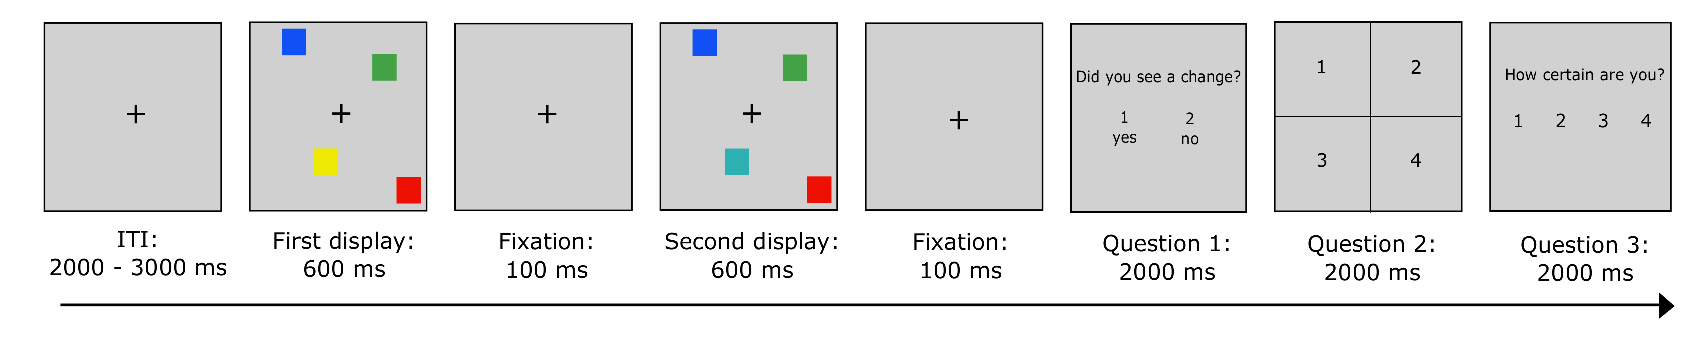
\includegraphics[width=1\textwidth]{paradigm_updated.eps}
	% figure caption is below the figure
	\caption{Caption 1}
	\label{fig:paradigm}       % Give a unique label
\end{figure*}



\subsection{Behavioural Analysis}

x
\subsection{EEG Data Acquisition}

x

\subsection{EEG Pre-processing}

x



\subsection{EEG Analysis}

x


\section{Behavioural Results}
\label{behaviouralresults}
\subsection{Accuracy and Difficulty}

x

\section{EEG Results}
\label{EEGresults}


x



\section{Discussion}
\label{discussion}
x


\begin{acknowledgements}
 x
\end{acknowledgements}


\section*{Conflict of Interest Statement}

The authors declare that the research was conducted in the absence of any commercial or financial relationships that could be construed as a potential conflict of interest.

\section*{Data Accessibility Statement}
The raw and pre-processed data can be found on the Open Science Framework:  

% BibTeX users please use one of
%\bibliographystyle{spbasic}      % basic style, author-year citations
%\bibliographystyle{spmpsci}      % mathematics and physical sciences
%\bibliographystyle{spphys}       % APS-like style for physics
%\bibliography{CBEEGPaper1}   % name your BibTeX data base



% Non-BibTeX users please use


\begin{thebibliography}{48}
\providecommand{\natexlab}[1]{#1}
\providecommand{\url}[1]{{#1}}
\providecommand{\urlprefix}{URL }
\expandafter\ifx\csname urlstyle\endcsname\relax
  \providecommand{\doi}[1]{DOI~\discretionary{}{}{}#1}\else
  \providecommand{\doi}{DOI~\discretionary{}{}{}\begingroup
  \urlstyle{rm}\Url}\fi
\providecommand{\eprint}[2][]{\url{#2}}

\bibitem[{Ball and Busch(2015)}]{ball_change_2015}
Ball F, Busch NA (2015) Change detection on a hunch: {Pre}-attentive vision
  allows sensing of unique feature changes. Attention, Perception, \&
  Psychophysics 77(8):2570--2588, \doi{10.3758/s13414-015-0963-9},
  \urlprefix\url{https://doi.org/10.3758/s13414-015-0963-9}

\bibitem[{Busch et~al.(2009)Busch, Fr\"und, and
  Herrmann}]{busch_electrophysiological_2009}
Busch NA, Fr\"und I, Herrmann CS (2009) Electrophysiological {Evidence} for
  {Different} {Types} of {Change} {Detection} and {Change} {Blindness}. Journal
  of Cognitive Neuroscience 22(8):1852--1869, \doi{10.1162/jocn.2009.21294},
  \urlprefix\url{https://doi.org/10.1162/jocn.2009.21294}

\bibitem[{Busch et~al.(2010)Busch, D\"urschmid, and Herrmann}]{busch_erp_2010}
Busch NA, D\"urschmid S, Herrmann CS (2010) {ERP} effects of change
  localization, change identification, and change blindness:. NeuroReport
  21(5):371--375, \doi{10.1097/WNR.0b013e3283378379},
  \urlprefix\url{https://insights.ovid.com/crossref?an=00001756-201003310-00011}

\bibitem[{Chetverikov et~al.(2018)Chetverikov, Kuvaldina, MacInnes,
  J\'ohannesson, and Kristj\'ansson}]{chetverikov_implicit_2018}
Chetverikov A, Kuvaldina M, MacInnes WJ, J\'ohannesson \'OI, Kristj\'ansson \'A
  (2018) Implicit processing during change blindness revealed with
  mouse-contingent and gaze-contingent displays. Attention, Perception, \&
  Psychophysics 80(4):844--859, \doi{10.3758/s13414-017-1468-5},
  \urlprefix\url{http://link.springer.com/10.3758/s13414-017-1468-5}


\end{thebibliography}

% and use \bibitem to create references. Consult the Instructions
% for authors for reference list style.
%
%\bibitem{RefJ}
% Format for Journal Reference
%Author, Article title, Journal, Volume, page numbers (year)
% Format for books
%\bibitem{RefB}
%Author, Book title, page numbers. Publisher, place (year)
% etc
%\end{thebibliography}

\end{document}
% end of file template.tex

